\documentclass[11pt,class=report,crop=false]{standalone}
\usepackage[screen]{../python}


\begin{document}


%====================================================================
\chapitre{Suites arithmétiques -- Suites géométriques}
%====================================================================

\objectifs{Tu vas manipuler deux types de suites fondamentales : les suites
arithmétiques et les suites géométriques.}


%%%%%%%%%%%%%%%%%%%%%%%%%%%%%%%%%%%%%%%%%%%%%%%%%%%%%%%%%%%%%%%%
%%%%%%%%%%%%%%%%%%%%%%%%%%%%%%%%%%%%%%%%%%%%%%%%%%%%%%%%%%%%%%%%

\begin{cours}[Suites arithmétiques]

\index{suite!arithmetique@arithmétique}

\objectifs{Une suite arithmétique est une suite telle que la différence entre deux termes consécutifs ait toujours la même valeur.}

\myfigure{0.8}{
\tikzinput{fig-suites-1}
}

\begin{enumerate}
  \item \textbf{Définition.} Une suite $(u_n)_{n\in\Nn}$ est une \defi{suite arithmétique} de \defi{raison} $r$ si on a $u_{n+1} = u_n + r$ pour tout $n\ge0$.
  

  
  \item \textbf{Formule de récurrence.} Une suite arithmétique est donc entièrement définie par son premier terme $u_0$ et sa raison $r$ :
  
  \mybox{terme initial $u_0$ et \\
  formule de récurrence $u_{n+1} = u_n + r$}


  
  \item \textbf{Formule directe.} On calcule $u_n$ directement par la formule :
  \mybox{$u_n = n r + u_0$} 
  
  
  \item \textbf{Exemple.}
  $$7 \quad 10 \quad 13 \quad 16 \quad 19 \quad \ldots$$
  C'est la suite arithmétique de terme initial $u_0 = 7$ et de raison $r=3$.
  La formule directe est $u_n = 3n + 7$.
  
  \item \textbf{Somme.} La somme des termes de $u_0$ jusqu'à $u_n$ est donnée par la formule :
  $$S_n = u_0 + u_1 + u_2 + \cdots + u_n = (n+1)u_0+ \frac{n(n+1)}{2}r$$
\end{enumerate}  
\end{cours}


%%%%%%%%%%%%%%%%%%%%%%%%%%%%%%%%%%%%%%%%%%%%%%%%%%%%%%%%%%%%%%%%
% Activité 1
%%%%%%%%%%%%%%%%%%%%%%%%%%%%%%%%%%%%%%%%%%%%%%%%%%%%%%%%%%%%%%%%


\begin{activite}[Suites arithmétiques]

\objectifs{Objectifs : programmer les différentes formules autour des suites arithmétiques.}

\begin{enumerate}
  \item Programme une fonction \ci{arithmetique_1(n,u0,r)} qui renvoie le terme de rang $n$ de la suite arithmétique définie par le terme initial $u_0$ et la raison $r$, en utilisant la formule de récurrence.
  Quel est le terme $u_{100}$ de la suite arithmétique définie par $u_0 = 13$ et $r=5$ ?
  
  \item Programme une fonction \ci{arithmetique_2(n,u0,r)} qui fait la même chose mais en utilisant cette fois la formule directe.
  
  \item Programme une fonction \ci{liste_arithmetique(n,u0,r)} qui renvoie la liste des termes $[u_0,u_1,u_2,\ldots,u_n]$.
  
  \item Programme une fonction \ci{est_arithmetique(liste)} qui teste si les termes $[u_0,u_1,u_2,\ldots,u_n]$ de la liste donnée forment le début d'une suite arithmétique.
  
  \emph{Indications.} 
  \begin{itemize}
    \item Le programme renvoie \ci{True} ou \ci{False}.
    \item On suppose que la liste contient au moins deux éléments.
    \item Si la liste est constituée des premiers termes d'une suite arithmétique alors, le terme initial est $u_0$ et la raison est $r= u_1-u_0$. 
    Et on doit avoir $u_{n+1}-u_n = r$ pour tout $n$. Tu peux alors utiliser la question précédente.   
    \item Exemple : avec $[3,5,7,10]$ la fonction renvoie \og{}Faux\fg{}.
  \end{itemize}
  
  \item Programme une fonction \ci{somme_arithmetique_1(n,u0,r)} 
  qui calcule, en additionnant les éléments, la somme des termes de rang $0$ à $n$ d'une suite arithmétique de terme initial $u_0$ et de raison $r$. 
Retrouve le même résultat par une fonction \ci{somme_arithmetique_2(n,u0,r)} 
qui utilise la formule de la somme donnée dans le cours ci-dessus.

Combien vaut la somme :
$$2+4+6+8+\cdots + 1000 \ ?$$
  
\end{enumerate} 
\end{activite}



%%%%%%%%%%%%%%%%%%%%%%%%%%%%%%%%%%%%%%%%%%%%%%%%%%%%%%%%%%%%%%%%
% Activité 2
%%%%%%%%%%%%%%%%%%%%%%%%%%%%%%%%%%%%%%%%%%%%%%%%%%%%%%%%%%%%%%%%


\begin{activite}[Trois termes d'une suite arithmétique]

\objectifs{Objectifs : déterminer si dans une liste donnée il existe trois termes d'une suite arithmétique.}

On te donne une liste ordonnée $[u_0,u_1,u_2,\ldots,u_n]$. Tu dois déterminer si dans cette liste on peut trouver trois termes $u_i,u_j,u_k$ qui font partie d'une suite arithmétique. Autrement dit, tels que :
$$u_i = u_j - r \quad u_k = u_j+r \quad \text{ pour un certain } r.$$


\myfigure{0.8}{
\tikzinput{fig-suites-3}
}

Par exemple dans la liste :
$$[10,11,13,17,19,20,23,29,31]$$
les trois termes $u_i = 11$, $u_j=17$, $u_k=23$ sont en progression arithmétique, de raison $r = 6$.

Programme l'algorithme ci-dessous en une fonction \ci{chercher_arithmetique(u)}
qui à partir d'une liste de termes \ci{u} renvoie trois termes en progression arithmétique (ou \ci{None} s'il n'y en a pas).


\bigskip

Le principe de l'algorithme est le suivant. Pour chaque élément $u_j$ de la suite (qui va jouer le rôle du potentiel élément central) :
\begin{itemize}
  
  \item On cherche un élément $u_i$ de rang $i$ plus petit que $j$ et un élément $u_k$ de rang $k$ plus grand que $j$ avec $u_j-u_i = u_k-u_j$ (on aura alors $u_j = u_i + r$ puis $u_k = u_j + r$).  Si on a cette égalité alors c'est gagné !
  
  \item Si on n'a pas cette égalité alors on prend un $i$ plus petit ou bien un $k$ plus grand.
  
\end{itemize} 

\bigskip

\begin{algorithme}
  \sauteligne 
 \begin{itemize}
   \item
   \begin{itemize}
     \item Entrée : une liste de termes $[u_0,u_1,\ldots,u_n]$ ordonnée.
     \item Sortie : trois termes en progression arithmétique (ou rien s'il n'y en pas).
   \end{itemize}

  \item Pour $j$ parcourant les indices de $1$ à $n-1$ :
  
   \begin{itemize}
     \item Poser $i=j-1$, $k=j+1$.
          
     \item Tant que $i \ge 0$ et $k \le n$ :
       \begin{itemize}
         \item Si $u_j-u_i = u_k-u_j$ renvoyer le triplet $u_i,u_j,u_k$ (qui forme une progression arithmétique). Le programme s'arrête là avec succès.
         \item Si $u_j-u_i < u_k-u_j$ alors faire $i \leftarrow i-1$.
         \item Si $u_j-u_i > u_k-u_j$ alors faire $k \leftarrow k+1$.
       \end{itemize}
     \end{itemize}   
   \item Lorsque la boucle \og{}pour\fg{} se termine sans avoir obtenu de triplet, c'est qu'il n'y en a pas.
   
 \end{itemize}  
 \end{algorithme}


\end{activite}

%%%%%%%%%%%%%%%%%%%%%%%%%%%%%%%%%%%%%%%%%%%%%%%%%%%%%%%%%%%%%%%%
%%%%%%%%%%%%%%%%%%%%%%%%%%%%%%%%%%%%%%%%%%%%%%%%%%%%%%%%%%%%%%%%

\begin{cours}[Suites géométriques]

\index{suite!geometrique@géométrique}

\objectifs{Pour une suite géométrique le quotient entre deux termes consécutifs est toujours le même.}

\myfigure{0.8}{
\tikzinput{fig-suites-2}
}

\begin{enumerate}
  \item \textbf{Définition.} Une suite $(u_n)_{n\in\Nn}$ est une \defi{suite géométrique} de \defi{raison} $q$ si on a $u_{n+1} = q u_n$ pour tout $n\ge0$.
  

  
  \item \textbf{Formule de récurrence.} Une suite géométrique est donc entièrement définie par son premier terme $u_0$ et sa raison $q$ :
  
  \mybox{terme initial $u_0$ et \\
  formule de récurrence $u_{n+1} = q u_n$}


  
  \item \textbf{Formule directe.} On calcule $u_n$ directement par la formule :
  \mybox{$u_n = u_0 \cdot q^n$} 
  
  
  \item \textbf{Exemple.}
  $$2 \quad 6 \quad 18 \quad 54 \quad 162 \quad \ldots$$
  est le début de la suite géométrique de terme initial $u_0 = 2$, de raison $q=3$. La formule directe est $u_n = 2 \times 3^n$.
  
  \item \textbf{Somme.} La somme des termes de $u_0$ jusqu'à $u_n$ (pour $q\neq1$)  est donnée par la formule :
  \mybox{$S_n = u_0 + u_1 + u_2 + \cdots + u_n = u_0 \times \dfrac{1-q^{n+1}}{1-q}$}
  que l'on mémorise par :
  $$\text{somme suite géométrique} = \text{terme initial} \times \frac{1 - \text{raison}^{\text{nombre de termes}}}{1-\text{raison}}$$
\end{enumerate}  
\end{cours}


%%%%%%%%%%%%%%%%%%%%%%%%%%%%%%%%%%%%%%%%%%%%%%%%%%%%%%%%%%%%%%%%
% Activité 3
%%%%%%%%%%%%%%%%%%%%%%%%%%%%%%%%%%%%%%%%%%%%%%%%%%%%%%%%%%%%%%%%


\begin{activite}[Suites géométriques]

\objectifs{Objectifs : refaire la première activité sur les suites arithmétiques, mais cette fois pour les suites géométriques.}

\begin{enumerate}
  \item Programme une fonction \ci{geometrique_1(n,u0,q)} qui renvoie le terme de rang $n$ de la suite géométrique définie par le terme initial $u_0$ et la raison $q$, en utilisant la formule de récurrence.
  Quel est le terme $u_{10}$ de la suite géométrique définie par $u_0 = 13$ et $r=5$ ?
  
  \item Programme une fonction \ci{geometrique_2(n,u0,q)} qui fait la même chose mais en utilisant cette fois la formule directe.
  
  \item Programme une fonction \ci{liste_geometrique(n,u0,q)} qui renvoie la liste des termes $[u_0,u_1,u_2,\ldots,u_n]$.
  
  \item Programme une fonction \ci{est_geometrique(liste)} qui teste si les termes $[u_0,u_1,u_2,\ldots,u_n]$ de la liste donnée forment le début d'une suite géométrique. 
  
  \emph{Indications.} 
 Si la liste est constituée des premiers termes d'une suite géométrique alors,  $\frac{u_{n+1}}{u_n} = \frac{u_1}{u_0}$ pour tout $n$. Utilise la question précédente.
 
  \item Programme une fonction \ci{somme_geometrique_1(n,u0,q)} 
  qui calcule, en additionnant les éléments, la somme des termes de rang $0$ à $n$ d'une suite géométrique de terme initial $u_0$ et de raison $q$. 
Retrouve le même résultat par une fonction \ci{somme_geometrique_2(n,u0,q)} 
qui utilise la formule de la somme donnée dans le cours ci-dessus.

Vers quelle valeur a l'air de tendre la somme :
$$1+\frac12+\frac14+\frac18+\frac1{16} + \cdots +\frac{1}{2^n}$$
lorsque $n$ tend vers l'infini ?
  
\end{enumerate} 
\end{activite}




%%%%%%%%%%%%%%%%%%%%%%%%%%%%%%%%%%%%%%%%%%%%%%%%%%%%%%%%%%%%%%%%
% Activité 4
%%%%%%%%%%%%%%%%%%%%%%%%%%%%%%%%%%%%%%%%%%%%%%%%%%%%%%%%%%%%%%%%


\begin{activite}[Tracer la somme d'une suite géométrique]

\objectifs{Objectifs : illustrer géométriquement la formule de la somme d'une suite géométrique.}

Voici un découpage d'un carré de côté $1$ qui illustre la formule :
$$\frac12 + \frac14 + \frac18 + \frac1{16} + \cdots + \frac{1}{2^n}
= 1 - \frac{1}{2^n}$$
\myfigure{0.7}{
\tikzinput{fig-carre-1}
}


\begin{enumerate}
  \item Programme une fonction \ci{affiche_un_carre(longueur)} qui affiche un carré de la longueur donnée. Utilise la tortue accessible depuis le module \ci{turtle}.\index{tortue}
  
   
  \item Programme une fonction \ci{affiche_un_rectangle(longueur)} qui trace un rectangle de hauteur la moitié de sa longueur. Il coupe le carré précédent en deux parties égales. 
  
  \item Programme une fonction \ci{affiche_les_carres(n)} qui construit notre figure.
  
  \emph{Indications.}
  \begin{itemize}
    \item Par exemple, on commence par tracer un carré de longueur $256$,
    \item on trace un rectangle qui coupe le carré en deux,
    \item puis on trace un carré de longueur $128$,
    \item puis on le découpe en deux, etc.
  \end{itemize}
  
\end{enumerate} 

De gauche à droite : le carré initial ; le carré coupé en deux rectangles ; un petit carré ; un découpage itéré.

\begin{center}
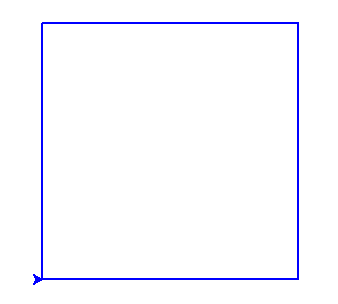
\includegraphics[scale=\myscale,scale=0.3]{ecran-carre-0}\qquad
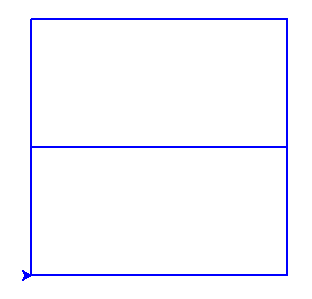
\includegraphics[scale=\myscale,scale=0.3]{ecran-carre-1}\qquad
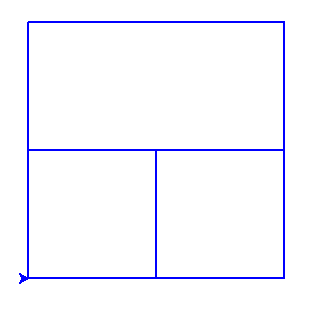
\includegraphics[scale=\myscale,scale=0.3]{ecran-carre-2}\qquad
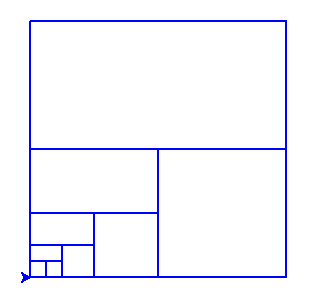
\includegraphics[scale=\myscale,scale=0.3]{ecran-carre-8}
\end{center}


\bigskip

\textbf{Preuves de la formule.}

On considère la suite : 
$$\frac12 \quad \frac14 \quad \frac18 \quad \frac1{16} \quad \cdots \quad \frac{1}{2^n} \quad \cdots$$
C'est la suite géométrique $(u_n)$ de terme initial $u_0 = \frac12$ et de raison $q=\frac12$.


\textbf{Preuve par le dessin.}

Le grand carré a pour aire $1$, l'aire totale des zones
\couleurnb{rouges}{non hachurées} est $\frac12 + \frac14  + \cdots + \frac{1}{2^n}$.
La zone hachurée \couleurnb{bleue }{}a pour aire $\frac{1}{2^n}$. 
Les zones \couleurnb{rouges et bleues }{}recouvrent tout le carré, donc leur aire totale vaut $1$. Ce qui prouve la formule annoncée :
$$\underbrace{\frac12 + \frac14 + \frac18 + \frac1{16} + \cdots + \frac{1}{2^n}}_{\text{\couleurnb{aire rouge}{aire non hachurée}}} \quad + \quad \underbrace{\quad \frac{1}{2^n} \quad}_{\text{\couleurnb{aire bleue}{aire hachurée}}}
= \underbrace{\qquad 1 \qquad}_{\text{aire du grand carré}}$$

\bigskip

\textbf{Preuve par le calcul.}

La formule pour la somme est 
$$S_{n-1} = u_0 + u_1 + u_2 + \cdots + u_{n-1} = u_0 \times \dfrac{1-q^{n}}{1-q}$$
(attention il y a bien $n$ termes dans la somme) et donc ici :
$$S_{n-1} =\frac12 + \frac14 + \frac18 + \frac1{16} + \cdots + \frac{1}{2^n}
= \frac12 \times \frac{1 - \frac{1}{2^n}}{1-\frac12}
= 1 - \frac{1}{2^{n}}$$

\end{activite}



%%%%%%%%%%%%%%%%%%%%%%%%%%%%%%%%%%%%%%%%%%%%%%%%%%%%%%%%%%%%%%%%
% Activité 5
%%%%%%%%%%%%%%%%%%%%%%%%%%%%%%%%%%%%%%%%%%%%%%%%%%%%%%%%%%%%%%%%


\begin{activite}[Meilleure suite arithmétique]

\objectifs{Objectifs : on te donne une liste ordonnée, tu dois trouver la suite arithmétique qui approche le mieux possible cette liste.}

Qu'est ce que la meilleure suite arithmétique qui approche une liste de nombres donnés ? Par exemple pour la liste $[3, 6, 9, 11]$, on a envie de l'approcher par la progression arithmétique $[3,6,9,12]$.

On nous donne donc des termes $v_0,v_1,\ldots,v_n$ (ordonnés du plus petit au plus grand). On va chercher une progression arithmétique $u_0,u_1,\ldots,u_n$ telle
que 
$$d = |v_0-u_0| + |v_1-u_1| + |v_2-u_2| + \cdots + |v_n-u_n|$$
soit le plus petit possible.

On appelle $d$ la \defi{distance} entre $[v_0,v_1,\ldots,v_n]$
et $[u_0,u_1,\ldots,u_n]$.
Pour l'exemple donné, $[3, 6, 9, 11]$ approchée par $[3,6,9,12]$, la distance vaut $1$.


\begin{enumerate}
  \item \textbf{Distance.} Programme une fonction \ci{distance(u,v)} qui calcule la distance
 $$d = |v_0-u_0| + |v_1-u_1| + |v_2-u_2| + \cdots + |v_n-u_n|$$
 entre deux listes $u = [u_0,u_1,\ldots,u_n]$ et $v = [v_0,v_1,\ldots,v_n]$.
  
  \item \textbf{Meilleure constante.} On nous donne une liste $w = [w_0,w_1,\ldots,w_n]$, on cherche une constante $m$ qui approche au mieux toutes les valeurs de la liste, c'est-à-dire telle que 
 $$d = |w_0-m| + |w_1-m| + |w_2-m| + \cdots + |w_n-m|$$ 
soit le plus petit possible.

Un nombre $m$ qui convient est simplement la médiane de la liste !
Par exemple pour $[3, 6, 9, 11]$, la médiane est $m=7.5$ et on a
$$d = |3-7.5| + |6-7.5| + |9-7.5| + |11-7.5| = 11$$
et on ne peut pas faire moins.
  
  Écris une fonction \ci{calcule_mediane(liste)} qui calcule la valeur médiane des éléments d'une liste. Par définition, la moitié des valeurs est inférieure ou égale à la médiane, l'autre moitié est supérieure ou égale à la médiane.
  Voir le rappel de cours juste après cette activité pour ce calcul.
  
   
  \item \textbf{Meilleure suite.} On va maintenant résoudre notre problème initial.  On nous donne donc une liste  $v = [v_0,v_1,\ldots,v_n]$
 et on cherche une progression arithmétique $u = [u_0,u_1,\ldots,u_n]$.
 Pour trouver les $(u_i)$ on doit donc trouver un terme initial $u_0$
 et une raison $r$.
 
 \emph{Méthode.}
 \begin{itemize}
   \item On va d'abord trouver un $r$ approché qui convient bien par une méthode de balayage. On cherche le meilleur $r$ en commençant par $r=0$ puis, par petits pas on teste jusqu'à, par exemple, $r = 2(v_1-v_0)$.
   
   \item Pour chaque $r$, le terme initial $u_0$ qui convient est la médiane de 
   la liste $(v_i - ir)$. (Justification : il faut minimiser la somme des $|v_i-u_i| = |v_i - ir - u_0|$ ; $u_0$ est donc la médiane des $(v_i - ir)$.)
   
 \end{itemize}
 
 Programme l'algorithme suivant en une fonction \ci{balayage(v,N)} qui renvoie
 le terme initial $u_0$ et la raison $r$ d'une suite arithmétique qui approche au mieux $v = [v_0,v_1,\ldots,v_n]$. Le paramètre $N$ correspond à la précision du balayage (plus $N$ est grand, plus l'approximation sera bonne).
 \begin{algorithme}
  \sauteligne 
 \begin{itemize}
   \item
   \begin{itemize}
     \item Entrée : une liste ordonnée de termes $v = [v_0,v_1,\ldots,v_n]$ et un entier $N$.
     \item Sortie : un terme initial $u_0$ et une raison $r$.
   \end{itemize}

  \item Définir un pas  $p = 2\frac{v_1-v_0}{N}$ (ce sera le pas pour le balayage de $r$).
  
  \item Initialise une valeur $d_{\min}$ par une très grande valeur (par exemple
  $d_{\min} = 10\,000$), cette variable stockera la distance la plus petite rencontrée.
  Deux variables $r_{\min}$ et $u_{0,\min}$ mémoriseront les meilleurs $r$ et $u_0$ trouvés.
  
  \item Poser $r=0$.
  
  \item Pour $k$ allant de $0$ à $N+1$ :
  
   \begin{itemize}
     \item Calculer $u_0$ la médiane de $(v_i - ir)$ (pour $0 \le i \le n$).
     
     \item Définir $u$, la liste des premiers termes de la suite arithmétique de terme initial $u_0$ et de raison $r$ (tu peux utiliser la fonction \ci{liste_arithmetique(n,u0,r)} de la première activité).
     
     \item Calcule la distance $d$ entre les listes $u$ et $v$.
     
     \item Si $d < d_{\min}$ alors faire :
      $d_{\min} \leftarrow d$ ; $r_{\min} \leftarrow r$ et  $u_{0,\min} \leftarrow u_0$.
      
      \item Faire $r \leftarrow r + p$.
  \end{itemize}
   
   \item Renvoyer $u_{0,\min}$ et $r_{\min}$.   
 \end{itemize}  
 \end{algorithme}

 Quelle est la meilleure progression arithmétique pour approcher la liste 
 $[6,11,14,20,24,29,37]$ ?
 
 
\end{enumerate} 
\end{activite}


%%%%%%%%%%%%%%%%%%%%%%%%%%%%%%%%%%%%%%%%%%%%%%%%%%%%%%%%%%%%%%%%
%%%%%%%%%%%%%%%%%%%%%%%%%%%%%%%%%%%%%%%%%%%%%%%%%%%%%%%%%%%%%%%%

\begin{cours}[Médiane]
Par définition de la \defi{médiane}\index{mediane@médiane}, la moitié des valeurs sont inférieures ou égales à la médiane, l'autre moitié sont supérieures ou égales à la médiane.

Voici comment calculer la médiane. On note $n$ la longueur de la liste, on suppose que la liste est ordonnée (du plus petit au plus grand élément).
  \begin{itemize}
    \item \textbf{Cas $n$ impair.} La médiane est la valeur de la liste au rang $\frac{n-1}{2}$.    
    Exemple avec \ci{liste = [12,12,14,15,19]} :
    \begin{itemize}
      \item la longueur de la liste est $n=5$ (les indices vont de $0$ à $4$),
      \item l'indice du milieu est l'indice $2$,
      \item la médiane est la valeur \ci{liste[2]}, c'est donc $14$.
    \end{itemize}
    
    \item \textbf{Cas $n$ pair.} La médiane est la moyenne entre la valeur de la liste au rang $\frac{n}{2}-1$ et celle au rang $\frac{n}{2}$.
    Exemple avec \ci{liste = [13,14,19,20]} :
    \begin{itemize}
      \item la longueur de la liste est $n=4$ (les indices vont de $0$ à $3$),
      \item les indices du milieu sont $1$ et $2$,
      \item la médiane est la moyenne entre \ci{liste[1]} et \ci{liste[2]}, c'est donc $\frac{14+19}{2} = 16.5$.
    \end{itemize}    
   \end{itemize} 
   

\end{cours}
\end{document}
